\cleardoublepage

\chapter{Study 4}
\label{res:survey}

\textbf{{\large Sleep and dream habits in a sample of French students}}

\hfill Under review at \emph{Journal of Sleep Research}

\bigskip

Raphael Vallat\textsuperscript{1} (PhD candidate), Mickael Eskinazi\textsuperscript{1} (PhD), Alain Nicolas\textsuperscript{1,2} (M.D, PhD), Perrine Ruby\textsuperscript{1} (PhD)

\textsuperscript{1} Lyon Neuroscience Research Center, Brain Dynamics and Cognition team, INSERM UMRS 1028, CNRS UMR 5292, Université Claude Bernard Lyon 1, Université de Lyon, Lyon, France

\textsuperscript{2} Unité Michel Jouvet, Centre Hospitalier Le Vinatier, 95 boulevard Pinel, Lyon, France

\subsection*{Summary}
\label{res:survey:summary}

Several authors have drawn the attention to the risk of sleep difficulties during college years. However, sleep and dream habits have been scarcely documented in young adults. We collected such information in a sample of 1137 French college students (411 males). In average, the participants reported spending roughly 8 hours in bed during weekdays, 9 hours during the weekends, and 90.9\% reported no difficulty to fall asleep. The mean sleep agitation score reported was 3.3 ± 1.7 (1-to-10 scale). Less than 0.4\% of students reported to have sleep-walking episodes regularly but nearly 7\% reported regular sleep-talking episodes. About 10\% reported to often take a nap. In average, participants mentioned 3 dream reports per week, 14\% said they had frequent lucid dreams and 6\% reported frequent recurrent dreams. The clarity of dream memory was positively correlated with dream recall frequency. An academic field effect (humanities, science, medicine) has been found for sleep duration. By contrast, no DRF differences were observed between disciplines. We observed the well-known negative correlation between age and dream recall frequency despite a limited age range, as well as a gender effect for several sleep and dream parameters. As compared to men, women spent more time in bed and reported slightly more dreams. These results 1) suggest that the great majority of French college students do not suffer from sleep disturbances, 2) show a gender difference for several sleep parameters, 3) provide supplementary arguments in favor of a small but consistent gender effect regarding dream recall frequency.

\paragraph{Keywords}
Sleep habits, dream recall frequency, students, survey, epidemiology, gender differences

\subsection*{Introduction}
\label{res:survey:intro}

Recent years have witnessed a renewed interest in sleep and dreaming \citep{dijk_dreaming_2015}. However, epidemiological investigations in healthy subjects combining questions on both sleep and dream habits are relatively rare. Such surveys are yet necessary to establish and keep up to date sleep and dream norms in the general population.

Of particular interest is the college population, which is more at risk of suffering from sleep difficulties than the general population \citep{buboltz_sleep_2001, curcio_sleep_2006, forquer_sleep_2008, lund_sleep_2010}. Yet, there are few, up-to-date, data available on sleep habits of college students. This is especially true for the European college population since most epidemiological studies have been carried out on Americans (e.g. \citealp{lund_sleep_2010}).

By contrast, dream habits of college students have been more investigated, especially by Mickael Schredl who extensively reported the dream patterns of German students. Yet, most surveys on dream habits were conducted on psychology students \citep{schredl_factors_2003}, and are therefore not necessarily representative of the student population since there is a great majority of women in this academic field. This point is not negligible given that several studies suggest a gender effect in sleep and dream habits \citep{beck_insomnia_2013, schredl_gender_2008}. It is important to note however, that regarding DRF the effect was not always reproduced and the overall effect size is small.

The originality of our study is to provide recent (2016) sleep and dream habits from a large sample (n = 1137) of French college students (Lyon University) pertaining to various academic fields (i.e. humanities, sciences, medicine), and composed for one third by males (n = 411). The web questionnaire asked about habitual time of light extinction and awakening during the week and the week-end, ability to fall asleep, sleep agitation, nap frequency, sleepwalking, sleep-talking, dream recall frequency, clarity of dream content, frequency of lucid and recurrent dreams. In addition to the descriptive aim of the study, we expected to reproduce results reported in previous surveys such as the correlation between age and DRF \citep{schredl_dream_2008}, or between DRF and the clarity of the dream memory, and a gender effect on sleep and dream parameters.

\subsection*{Methods}
\label{res:survey:methods}

Data were collected in 2016 using an online questionnaire for the recruitment phase of an fMRI sleep study. The subjects were informed of the study through an announcement sent to several mailing lists of Lyon University. Among with basic sociodemographic variables (age, gender, height, weight, education, academic discipline), the online survey included the following questions:

\begin{my_list_num}
    \item What time do you usually go to bed and get up during weekdays?
    \item What time do you usually go to bed and get up during weekends?
    \item In general, you fall asleep: very easily, easily, quite easily, with difficulty or with great difficulty?
    \item On a scale of 1 to 10, how much agitated is your sleep? (1 = not at all agitated, 10 = very agitated)
    \item How often do you experience sleepwalking episode? (never, rarely, sometimes, often)
    \item How often do you talk during your sleep? (never, rarely, sometimes, often)
    \item How often do you take daytime nap? (never, rarely, sometimes, often)
    \item How many days per week do you usually wake up with a dream in mind?
    \item How many days per month do you usually wake up with a dream in mind?
    \item How often do you have lucid dream(s) (i.e. dreams in which you are aware that you are dreaming)? (never, rarely, sometimes, often)
    \item How often do you have recurrent dream(s) (i.e. dream experienced repeatedly)? (never, rarely, sometimes, often)
    \item In general, how clear is the memory of your dream content? (very vague, vague, clear, very clear)
\end{my_list_num}

We collected 1262 completed questionnaires (459 M, age range = 18 - 61 yr., mean age ± SD = 22.75 ± 3.94 yr.). In order to be representative of a student population, participants older than 30 years were removed, leading to a final sample size of 1137 (411M - 726 F, mean age ± SD  = 22.23 ± 2.36 yr., height = 170.2 ± 11.4 cm, weight = 64.1 ± 11.6 kg, education = 3.3 ± 1.8 years after high school).

A binomial logistic regression was performed to investigate the gender differences in sleep and dream habits. In order to be entered in the model, the frequency of sleepwalking and sleep-talking episodes, and the frequency of lucid and recurrent dreams were recoded as follows: Never → 0, Rarely → 1, Sometimes → 2, Often → 3. The dream clarity scale was recoded using: Very vague → 0, Vague → 1, Clear → 2, Very clear → 3.  The level of ease or difficulty to fall asleep was recoded using: very easily → 0, easily → 1, quite easily → 2, with difficulty → 3, with great difficulty → 4.

Finally, we compared the sleep and dream habits of students as a function of the academic discipline. We partitioned the sample in three broad categories, namely sciences (i.e. hard sciences and technology, n = 432 students), humanities (i.e. social sciences, literature, psychology, educational science, law school, n = 417 students) and medicine (i.e. medical and dental studies, n = 190). The 98 remaining students of the sample were not included in the analysis because they were issued from heterogeneous academic and/or professional environment.

\subsection*{Results}
\label{res:survey:results}

\subsubsection*{Sleep habits}
The average time in bed was 7.90 ± 0.96 hours (range = 3.5 - 12 hours) during weekdays and 9.10 ± 1.13 hours (range = 4 - 13 hours, paired t-test = <.001) during weekends. Sleep schedules during weekdays and weekends are reported in Fig 1. The peak bedtime was between 11 and 11.59 pm (43.4\%) during weekdays and between 0 and 0.59 am during weekends (33.57\%). The peak waking time was between 7 and 7.59 am during weekdays (42.33\%) and between 10 and 10.59 am during weekends (29.96\%).

\begin{figure}[htb]
	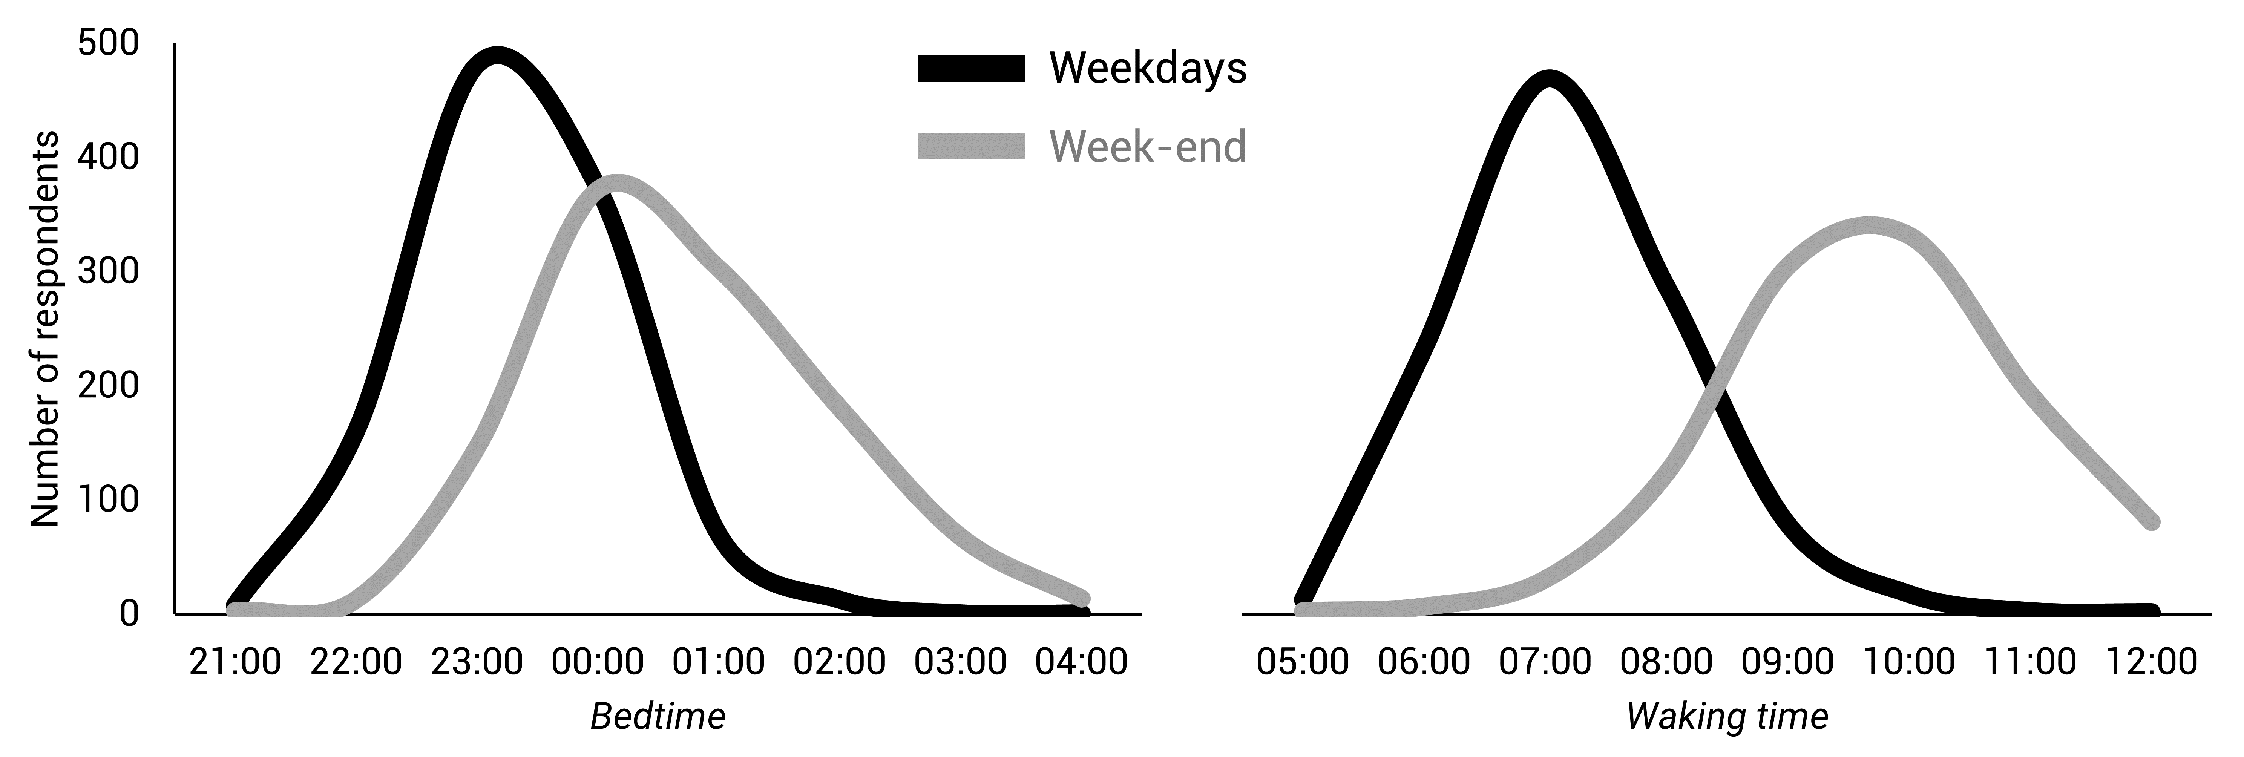
\includegraphics[width=\textwidth]{Fig/Results/Survey/Fig1.png}
	\caption*{\textbf{Fig 1.} Bedtime (left) and waking time (right) distribution during weekdays (black lines) and weekends (grey lines).}
\end{figure}

Only 4 respondents (0.35\%) reported having great difficulty falling asleep. Conversely, 429 students (37.7\%) reported falling asleep easily and 184 (16.18\%) reported falling asleep very easily. The mean sleep agitation score reported was low (3.3 ± 1.7). Regarding sleepwalking, only 4 students (0.35\%) reported having regular episodes, while 986 (86.72\%) of them reported never having episodes. The percentage of students reporting regular episodes of sleep-talking was higher (75 students, 6.6\%), and only 315 respondents (27.7\%) declared never having sleep-talking episodes. Finally, a total of 113 participants (9.94\%) reported that they often took nap, while 196 respondents (17.24\%) reported that they never took nap. Frequencies of nap, sleepwalking, sleep-talking, recurrent dreams and lucid dreams are reported in Fig 2.

\begin{figure}[htb]
	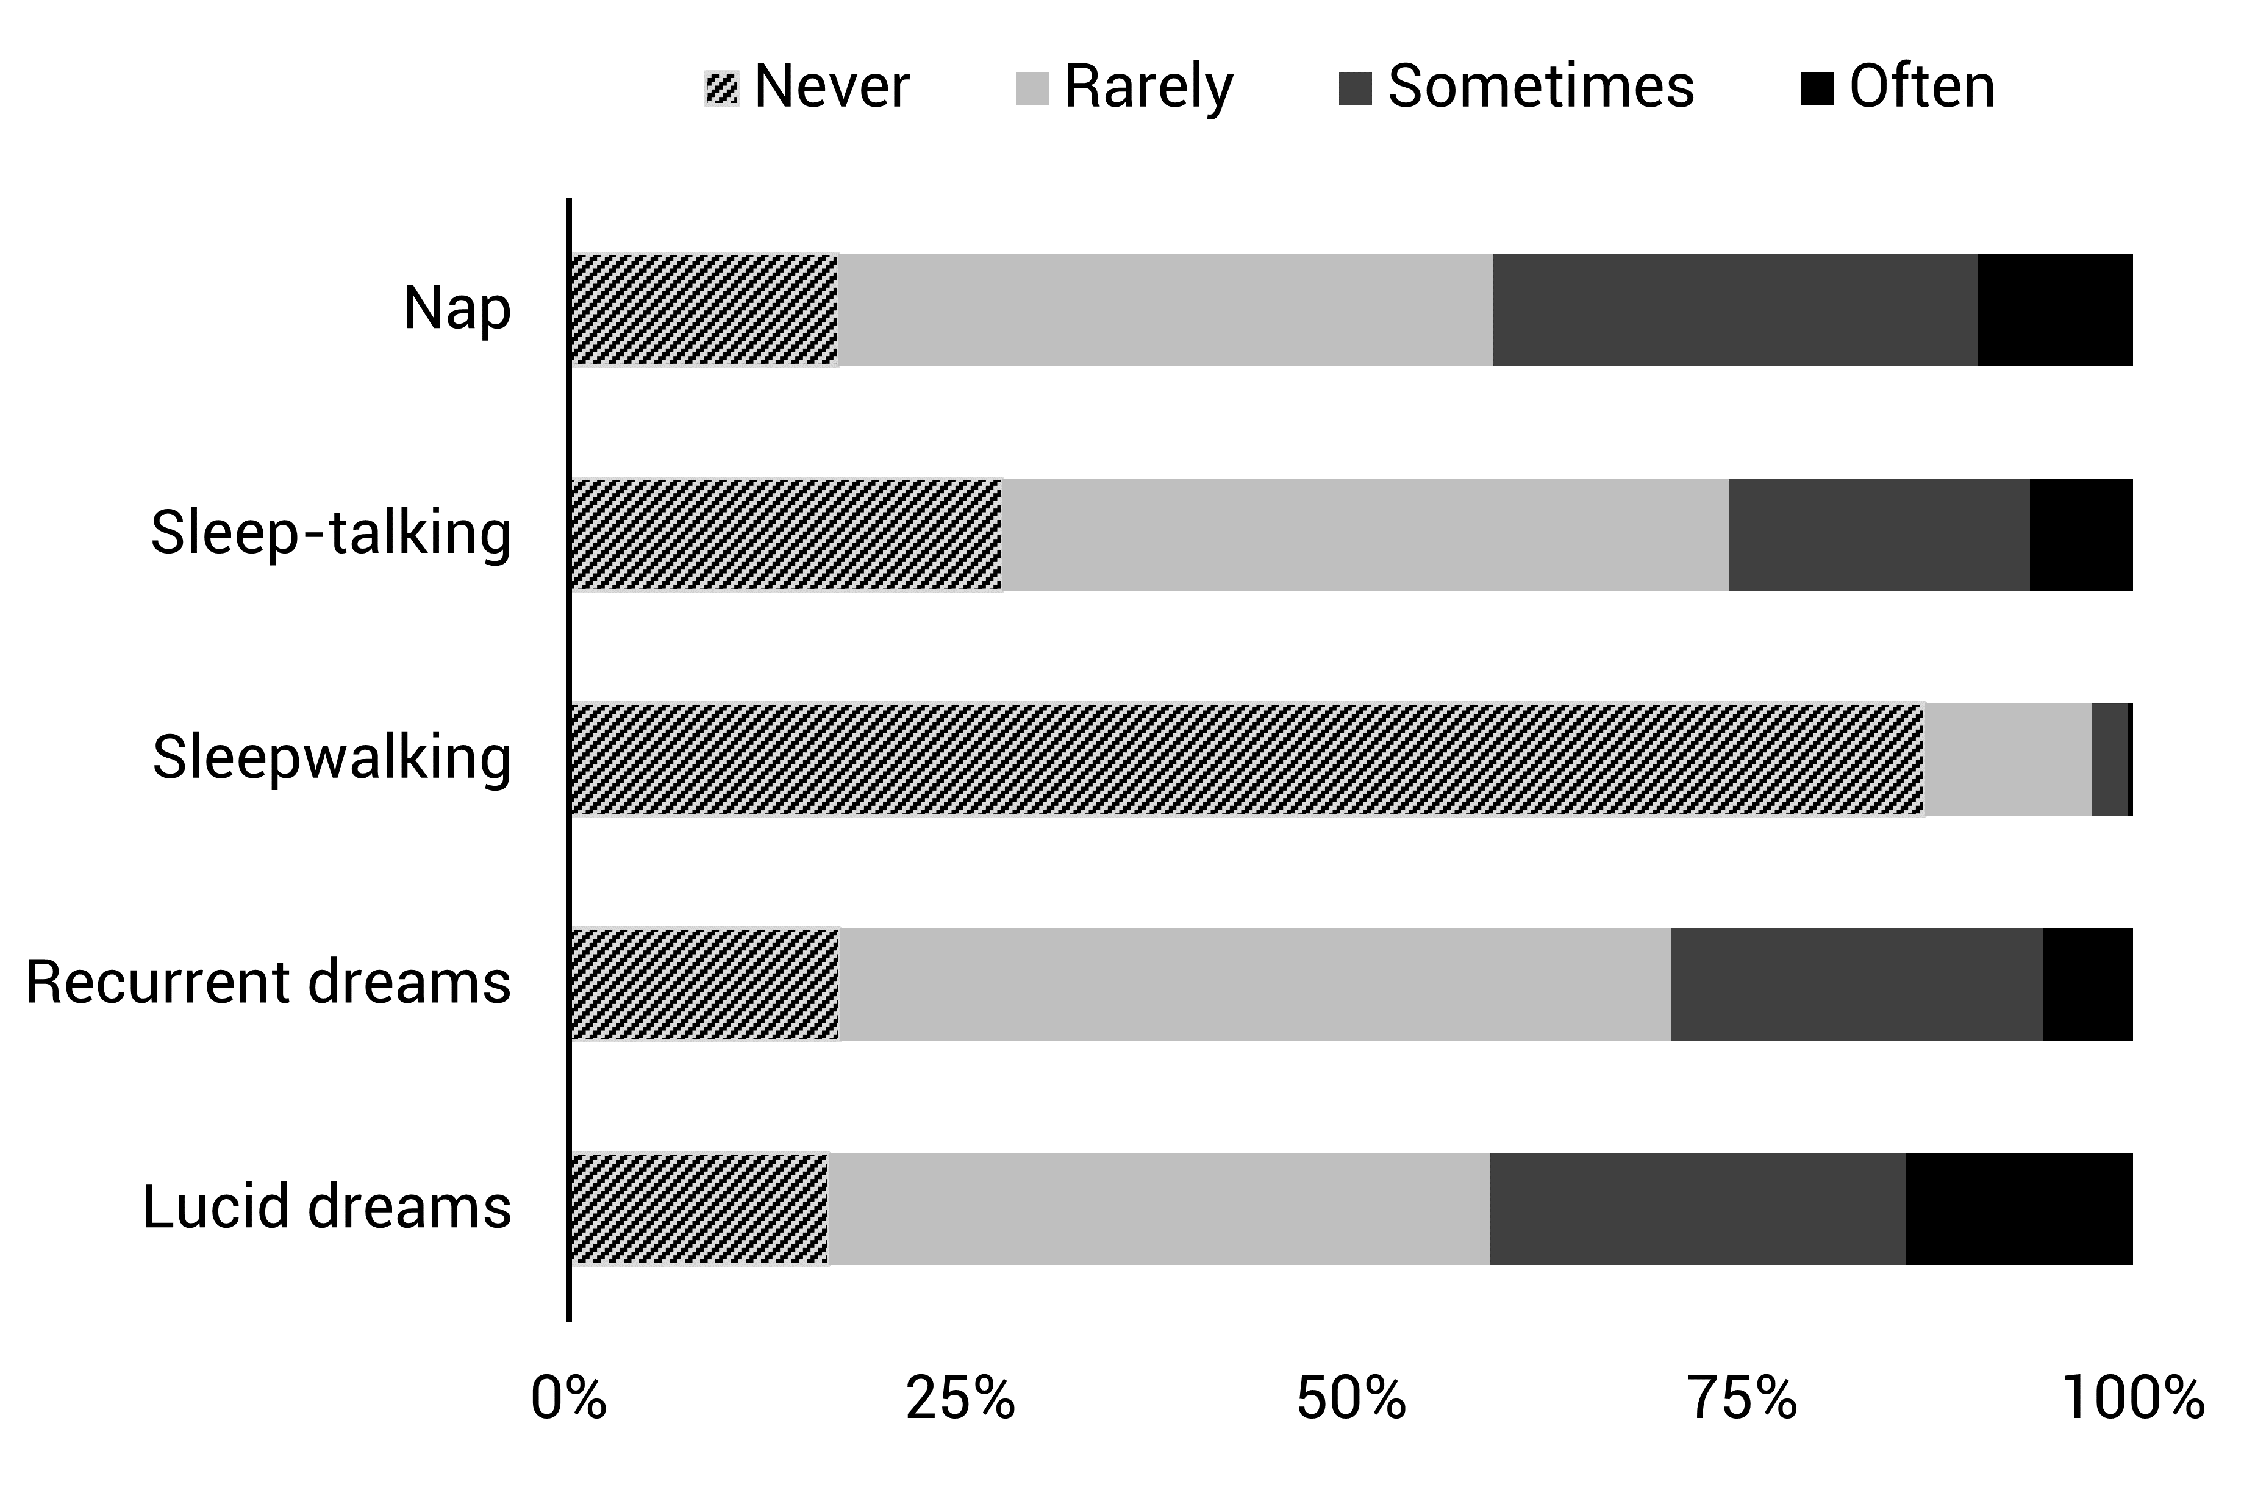
\includegraphics[width=\textwidth]{Fig/Results/Survey/Fig2.png}
	\caption*{\textbf{Fig 2.} Frequencies of nap, sleep-talking, sleepwalking, recurrent dreams and lucid dreams in the sample.}
\end{figure}

\subsubsection*{Dream recall frequency}
The mean dream recall frequency (DRF) was 3.12 ± 1.78 days per week (i.e. the participants recalled a dream in average 3 mornings per week) and 12.84 ± 7.51 days per month. Fifty-eight participants (5.10\%) reported not recalling any dream per week and 9 participants (0.79\%) reported not recalling any dream per month. On the opposite, 34 participants (2.99\%) reported recalling a dream 7 mornings per week and 29 participants (2.55\%) reported recalling a dream every morning of the month.

Despite the narrow age range of our sample (18 to 30 years old), we were able to evidence the negative correlation between DRF (weekly estimation) and age (Fig 3A) evidenced in previous studies with a larger range (e.g. \citealp{schredl_dream_2008}). Weekly DRF was positively correlated with the frequency of lucid dreams (Fig 3C), as could be expected from previous results \citep{stepansky_austrian_1998, schredl_lucid_2004, schredl_frequency_2011}. Weekly DRF was also positively correlated with the clarity of dreams (Fig 3D) and the level of agitation during sleep (Pearson r = 0.08, p = 0.008). We observed neither an effect of the academic field on DRF, nor a significant correlation between DRF and the education level (Fig 3B). These findings are consistent with two studies that reported no association between DRF and the education level and DRF and the socioeconomic status \citep{schredl_dream_2007, schredl_dream_2008}.

\begin{figure}[htb]
	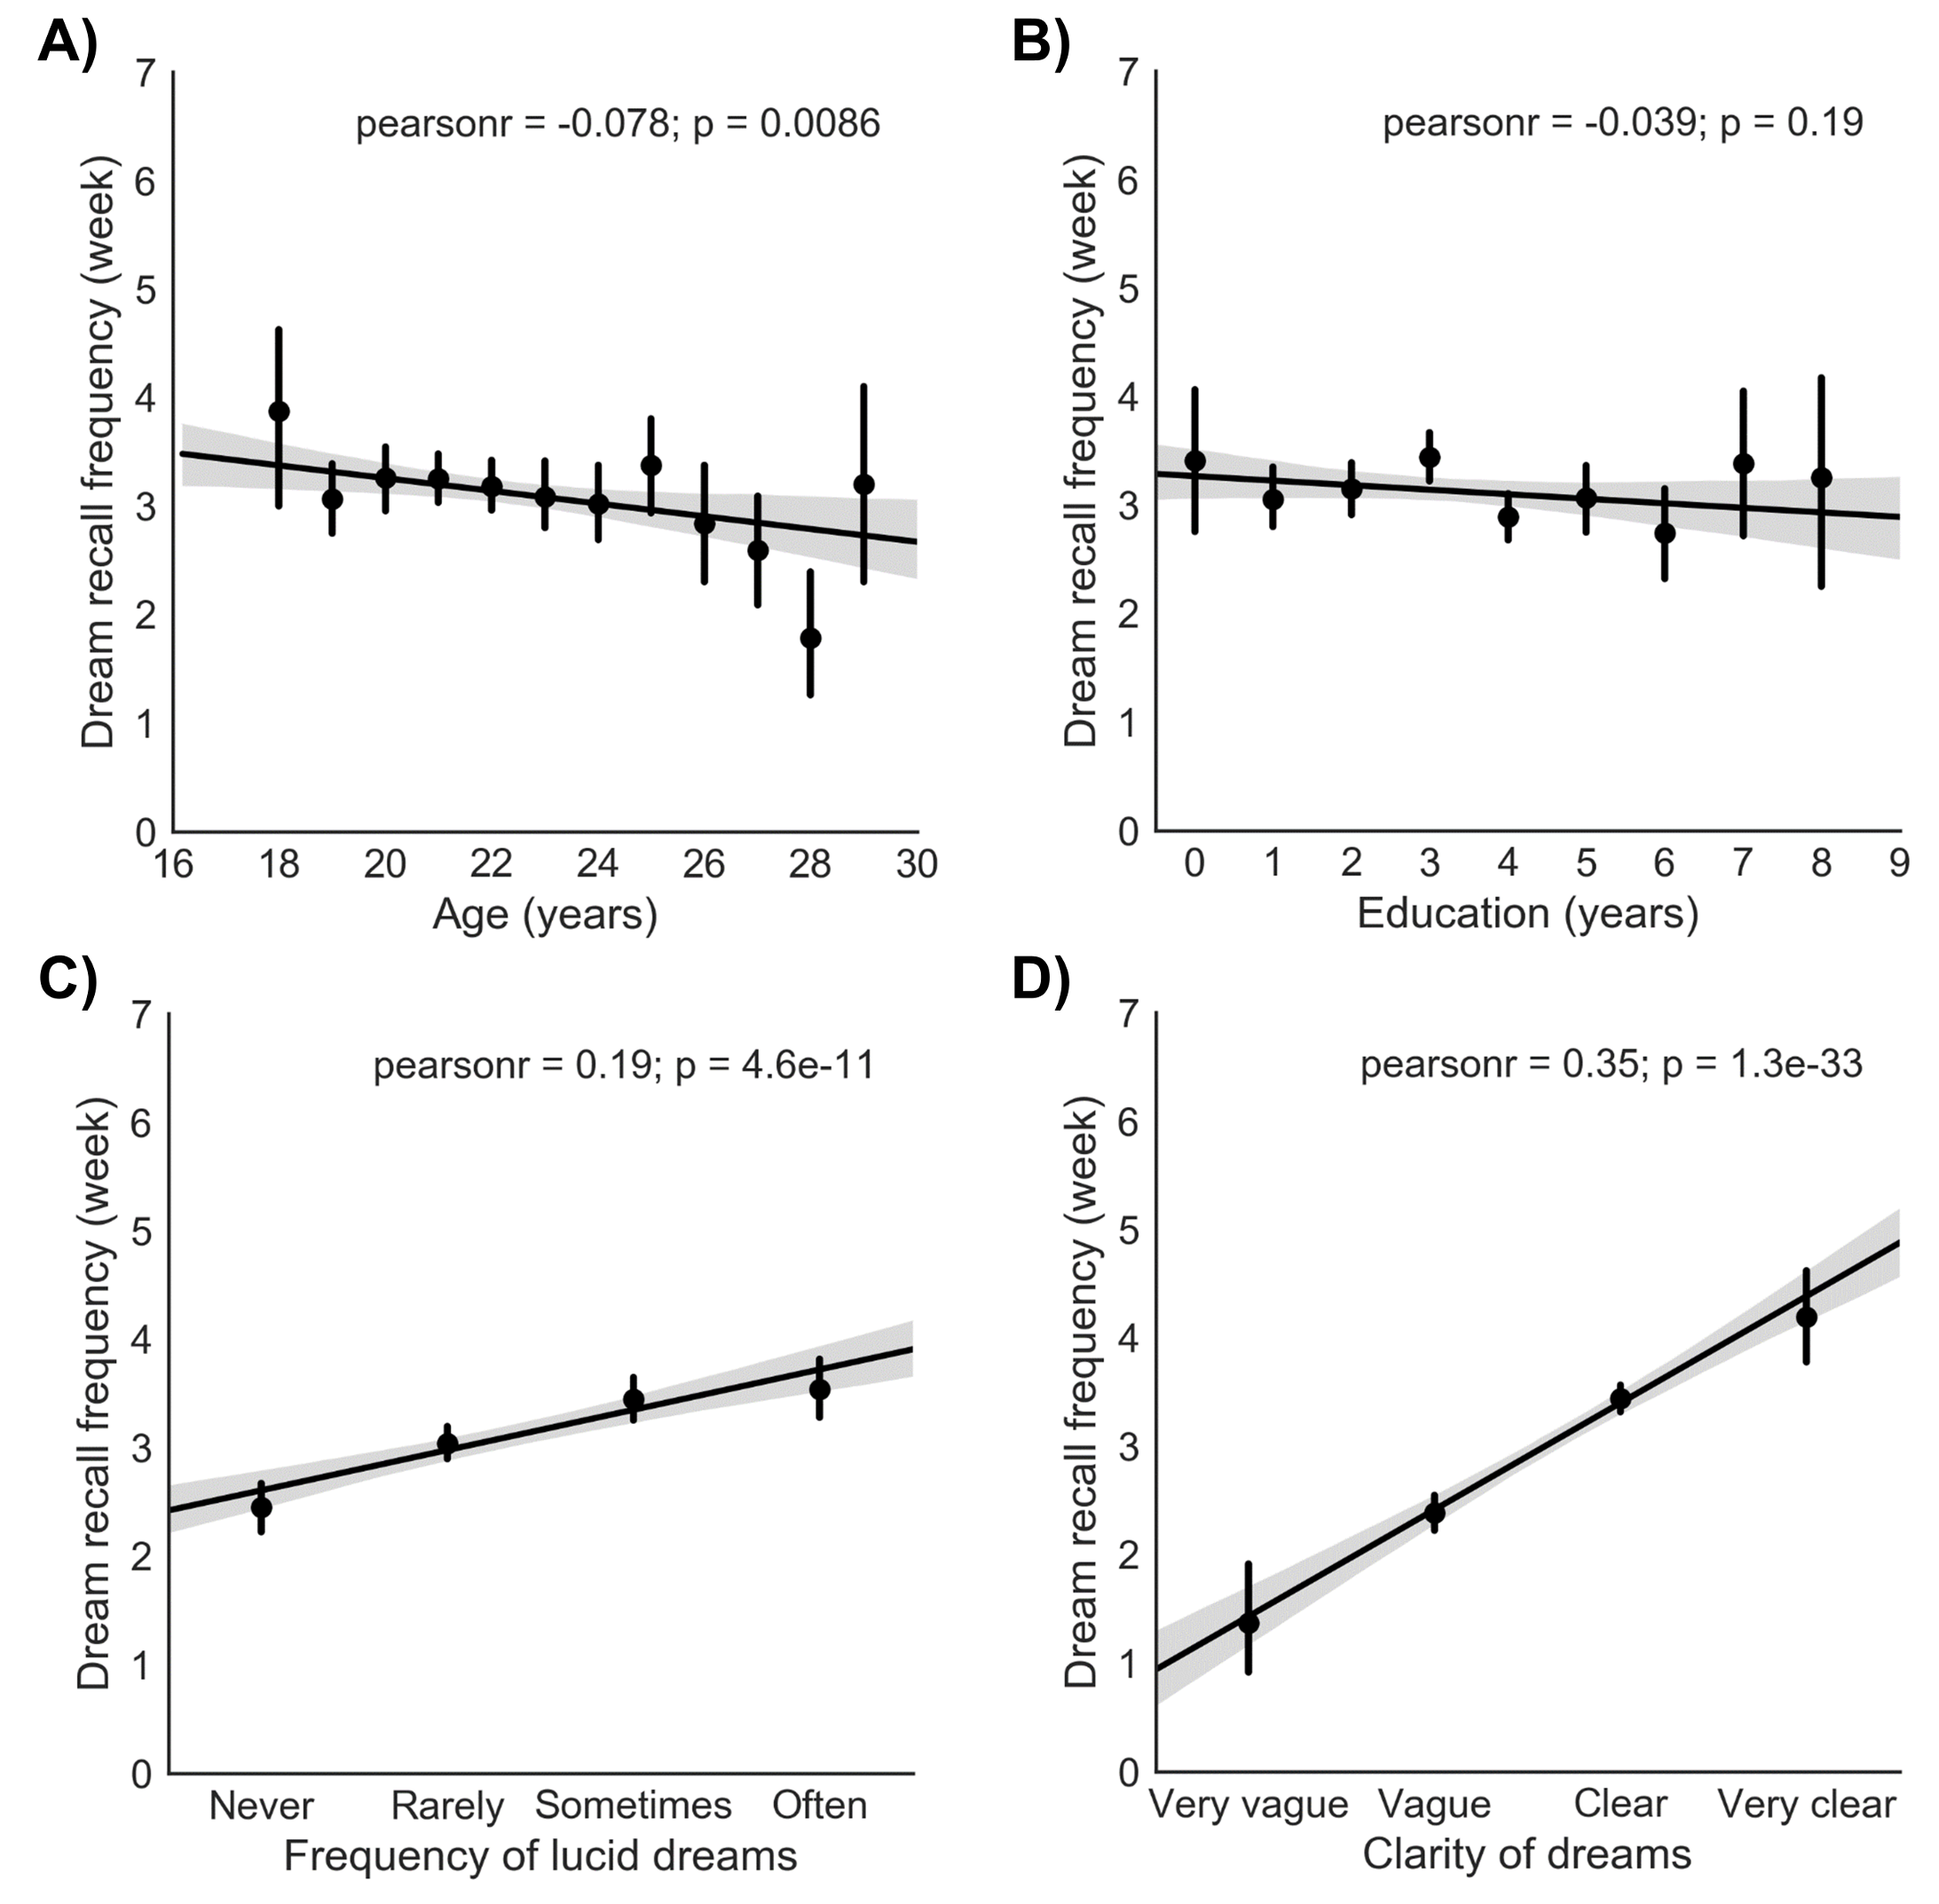
\includegraphics[width=\textwidth]{Fig/Results/Survey/Fig3.png}
	\caption*{\textbf{Fig 3.} Correlations between dream recall frequency (number of mornings per week with a dream in mind) and (A) age (B) education level (C) frequency of lucid dreams (D) clarity of dream memory. Error bars represent 95\% confidence intervals.}
\end{figure}

\paragraph{Clarity of dreams}
Thirty-five participants (3.08\%) reported that the usual clarity of their dreams was very vague. By contrast, 75 participants (6.60\%) reported that their dreams were usually very clear. The great majority of respondents (n=705, 62.0\%) reported that their dreams were usually clear.

\paragraph{Frequency of lucid dreams}
A lucid dream is a dream during which the dreamer is aware of dreaming. In our sample, 165 participants (14.51\%) reported that they often had lucid dreams, while 189 participants (16.62\%) reported that they never had a lucid dream (Fig 2). From these figures, it could be inferred that approximatively 83\% of the participants have already experienced a lucid dream at least once. This number is remarkably consistent with those from other studies focusing on student population (e.g. 82\% in \citealp{schredl_lucid_2004}). However, it should be noted that the definition of lucid dreaming given in the questionnaire did not include the ability to control the dream characters and narratives, but simply to be aware of dreaming during the dream. It is generally admitted that control over the dream represents the full extent of lucid dreaming and is more difficult to attain than the mere awareness of dreaming \citep{purcell_dream_1986, laberge_exploring_1991}. Consequently, the proportion of participants having already experienced a lucid dream would probably be lower if the definition of lucid dreaming involved the ability to exert some degree of control over the dream.

\paragraph{Frequency of recurrent dreams}
A recurrent dream is a dream which is experienced repeatedly. In our sample, 65 participants (5.72\%) reported that they often had recurrent dreams, while 197 participants (17.33\%) reported that they never had a recurrent dream (Fig 2), meaning that roughly a little more than 80\% of the participants had already experienced recurrent dreams at some point in their lives. Again, this figure is consistent with several studies that reported a prevalence of 60\% to 75\% of recurrent dreams in college students and young adults \citep{zadra_recurrent_1996}.

\subsubsection*{Gender differences}
Table 1 depicts the summary of the binomial logistic regression for gender differences. In our sample, as compared to men, women spend more time in bed (during both weekdays and weekends), take naps more often, are more susceptible to have episodes of sleepwalking, and have a higher weekly-estimated DRF. Women tend also to have a more agitated sleep and to report more difficulties to fall asleep. Finally, the frequency of lucid dreams tends to be higher in men, while the frequency of recurrent dreams tends to be higher in women.

\begin{table}[!htb]
    \caption*{\textbf{Table 1. Binomial logistic regression for gender differences in sleep and dream habits (n=1137).} SE = standardized estimate, DRF = dream recall frequency. Frequencies of nap, sleepwalking, sleep-talking, recurrent dreams and lucid dreams are expressed using a recoded scale ranging from 0 (Never) to 3 (Often). Sleep agitation is scored on a 1-to-10 scale where 1 means no agitation at all during sleep and 10 means a very agitated sleep. Difficulty falling asleep is expressed using a recoded scale ranging from 0 (very easy to fall asleep) to 4 (very difficult to fall asleep). For sleep agitation and difficulty to fall asleep, higher scores indicate more disturbances.}
    \begin{tabularx}{\textwidth}{lllXXX}
    \toprule
    Variable                       & Men                       & Women         & SE    & X²    & p        \\ \midrule
    \emph{Sleep}                   &                           &               &       &       &          \\
    Time in bed (weekdays)         & 7.70 ± 1.0                & 8.02 ± 0.9    & 0.31  & 28.92 & .001     \\
    Time in bed (weekends)         & 8.93 ± 1.2                & 9.19 ± 1.1    & 0.13  & 5.14  & .023     \\
    Difficulty falling asleep      & 1.35 ± 0.9                & 1.42 ± 0.9    & 0.14  & 3.61  & .057     \\
    Sleep agitation                & 3.13 ± 1.6                & 3.39 ± 1.8    & 0.07  & 2.87  & .090     \\
    Frequency of nap               & 1.24 ± 0.9                & 1.39 ± 0.8    & 0.23  & 9.31  & .002     \\
    Frequency of sleepwalking      & 0.12 ± 0.4                & 0.19 ± 0.5    & 0.33  & 4.02  & .045     \\
    Frequency of sleep-talking     & 1.04 ± 0.9                & 1.05 ± 0.8    & -0.11 & 0.61  & 0.43     \\
    \emph{Dream}                   &                           &               &       &       &          \\
    DRF (weekly)                   & 2.83 ± 1.7                & 3.29 ± 1.8    & 0.10  & 15.50 & .001     \\
    DRF (monthly)                  & 11.60 ± 7.3               & 13.54 ± 7.5   & 0.01  & 0.18  & .663     \\
    Dream clarity                  & 1.69 ± 0.6                & 1.74 ± 0.6    & -0.04 & 0.16  & .689     \\
    Frequency of recurrent dreams  & 1.09 ± 0.8                & 1.23 ± 0.8    & 0.14  & 2.77  & .096     \\
    Frequency of lucid dreams      & 1.40 ± 0.9                & 1.38 ± 0.9    & -0.16 & 3.83  & .050     \\ \bottomrule
    \end{tabularx}%
\end{table}

\subsubsection*{Academic fields differences}
Table 2 depicts the results of the ANOVA testing an academic disciplines effect on sleep and dream variables (Science, n=432; Humanities, n=417; Medicine, n=190). First, the time in bed during weekdays was significantly different between the three groups. Post-hoc tests (two-sided T-tests) showed that humanities students reported a longer time in bed duration than students in sciences (T = 6.31, p < .001) or medicine (T = 2.81, p = .005). Second, medicine student reported less recurrent dreams than humanities (T = 2.49, p = .013) or sciences students (T = 2.27, p =.023).

However, there results should be taken cautiously considering that the average age of the students was slightly lower in the Science group (i.e. science students were significantly younger than humanities, T = 3.91, p < .001; and medicine students, T = 2.65, p = .008) and that a sex ratio difference has been observed between the three academic fields. Specifically, the proportion of females was higher in humanities than in science (Z = 15.02, p < .001) or medicine (Z = 6.29, p < .001), and was also higher in medicine than in science (Z = 7.23, p < .001). Since we have previously seen that women reported a higher time in bed duration and tended to have a higher frequency of recurrent dreams, the finding that humanities student spend more time in bed could be as least partly explained by a higher proportion of women in this academic discipline. Apart from the frequency of recurrent dreams, no difference was found regarding the other dream variables.

% Table column width
\newcolumntype{b}{>{\hsize=0.3\textwidth}X}

\begin{table}[!htb]
    \caption*{\textbf{Table 2. Sleep and dream habits differences between academic disciplines (Science, Humanities and Medicine)}. Differences between disciplines were assessed using one-way ANOVAs. Sex ratio difference between disciplines was assessed using a chi-squared test. DRF = dream recall frequency. Frequencies of nap, sleepwalking, sleep-talking, recurrent dreams and lucid dreams are expressed using a recoded scale ranging from 0 (Never) to 3 (Often). Sleep agitation is scored on a 1-to-10 scale where 1 means no agitation at all during sleep and 10 means a very agitated sleep. Difficulty to fall asleep is expressed using a recoded scale ranging from 0 (very easy to fall asleep) to 4 (very difficult to fall asleep). For sleep agitation and difficulty to fall asleep, higher scores indicate more sleep disturbances.}
    \begin{tabularx}{\textwidth}{bXXXll}
    \toprule
    Variable                       & Humanities & Science    & Medicine   & X²/F   & p    \\ \midrule
    Sex ratio (F/M)                & 3.8        & 1.1        & 1.7        & 67.5   & .001 \\
    Age                            & 22.4 ± 2.4 & 21.8 ± 2.0 & 22.3 ± 2.4 & 8.0    & .001 \\
    \emph{Sleep}                   &            &            &            &        &      \\
    Time in bed (weekdays)         & 8.1 ± 1.0  & 7.7 ± 0.9  & 7.9 ± 0.8  & 21.1   & .001 \\
    Time in bed (weekends)         & 9.1 ± 1.2  & 9.1 ± 1.2  & 9.1 ± 1.0  & 0.1    & .921 \\
    Ease/Difficulty to fall asleep & 1.4 ± 0.9  & 1.4 ± 0.8  & 1.3 ± 0.9  & 1.7    & .191 \\
    Sleep agitation                & 3.3 ± 1.8  & 3.3 ± 1.7  & 3.1 ± 1.7  & 0.7    & .522 \\
    Frequency of nap               & 1.3 ± 0.9  & 1.3 ± 0.9  & 1.4 ± 0.9  & 1.0    & .379 \\
    Frequency of sleepwalking      & 0.2 ± 0.5  & 0.2 ± 0.5  & 0.2 ± 0.4  & 0.2    & .808 \\
    Frequency of sleep-talking     & 1.0 ± 0.9  & 1.1 ± 0.9  & 1.0 ± 0.9  & 0.9    & .409 \\
    \emph{Dream}                   &            &            &            &        &      \\
    DRF (weekly)                   & 3.2 ± 1.8  & 3.1 ± 1.8  & 3.1 ± 1.8  & 0.3    & .733 \\
    DRF (monthly)                  & 12.9 ± 7.6 & 12.9 ± 7.6 & 12.6 ± 7.2 & 0.2    & .851 \\
    Dream clarity                  & 1.7 ± 0.6  & 1.8 ± 0.7  & 1.7 ± 0.6  & 0.9    & .424 \\
    Frequency of recurrent dreams  & 1.2 ± 0.8  & 1.2 ± 0.8  & 1.0 ± 0.7  & 3.4    & .035 \\
    Frequency of lucid dreams      & 1.4 ± 0.9  & 1.4 ± 0.9  & 1.4 ± 1.0  & 0.2    & .825 \\ \bottomrule
    \end{tabularx}
\end{table}

\subsection*{Discussion}
\label{res:survey:discussion}

Regarding sleep habits and patterns, our findings suggest that French college students have little or unfrequent sleep disturbances. For instance, the average time in bed during weekdays is almost one hour more in our study (7 h 54 min) than the one reported in a representative sample of Taiwanese students (6 h 59; \citealp{tsai_sleep_2004}), and is equivalent to two studies based on American students habits (8 h 2 min in \citealp{buboltz_sleep_2001}; 7 h 45 min in \citealp{lund_sleep_2010}). Note however that only the time in bed could be extracted from the participants’ answers (time spent in bed, both awake and sleeping). It follows that the sleep duration may be overestimated in our survey, even if probably not that much since the large majority of students (90.9\%) reported no difficulty to fall asleep

Consistent with several studies, we have found that the average time in bed was longer of more than one hour during weekends as compared to weekdays, suggesting that, to some extent, students suffer from sleep deprivation during the weekdays. Nevertheless, it is important to note that the average time in bed during both weekdays and weekends fall in the range that is considered as normal (i.e. 7-9 hours/night; \citealp{hirshkowitz_normal_2004}).

Women self-reported a longer time in bed, during weekdays (19 min more than men on average) and weekends (16 min more than men on average) as could be expected from a previous survey which assessed the French general population sleep habits \citep{beck_insomnia_2013}. \citet{reyner_gender-and_1995} reported results close to ours experimentally recording sleep with home-recorded logs in 400 British adults, i.e. an 18-min longer total sleep time in women. It is however interesting to note that in their sample, this effect was not significant in the \q{young} group (20-34 years) but appeared only in the older groups. In the same study, they also observed that women had a poorer subjective sleep quality and an increased intra-sleep wakefulness. A possible explanation for an increased time in bed in women could thus be that they spend more time in bed to compensate for increased intrasleep awakenings. In coherence with this hypothesis, in our sample women reported more difficulties to fall asleep, more agitation during sleep and a higher frequency of daytime naps.

Regarding dream recall, in average students reported having a dream 3 mornings per week, which is higher than what was observed in a representative sample of the German adult population \citep{schredl_dream_2008}, but similar to the figures reported in several studies with German student samples composed of a great majority of women (3.5 dream recalls per week in \citealp{schredl_reliability_2005}, N = 196 (138 women), age = 24.8 ± 5.9; 2.75 in \citealp{schredl_factors_2003},  N = 444 (376 women), age = 23.5 ± 5.70). The fact that the averaged DRF is not that much different in our sample with a more balanced sex ratio is probably due to the fact that the effect size of gender difference in DRF, when this effect is found, is generally small. Regarding the DRF discrepancy between student and the general adult population it is probably at least partly explained by the well-known negative correlation between DRF and age, which we were able to replicate in this study despite a narrow age range (18 to 30 years old). We also found a significant correlation between the clarity of the dream memory and DRF. This result is consistent with previous ones (e.g. \citealp{schredl_relationship_2000}) showing a significant correlation between dream report length and DRF and suggest that the more often you recall dreams the clearer they are.

Regarding gender difference, our results add to the numerous studies reporting a higher DRF in women than in men. This difference was reported to be lower during childhood, an observation that led \citep{schredl_gender_2008} to explain adults gender difference in DRF by a gender-specific dream socialization process. Their hypothesis is that girls are encouraged more often than boys to talk about their dreams, which could explain the gender effect since the interest in dream is known to increase DRF \citep{schredl_factors_2003}. However, there is currently a lack of longitudinal studies to support this hypothesis. Another explanation could relate to gender differences in sleep patterns. Indeed, we have mentioned previously that women tend to have increased intra-sleep wakefulness and poorer sleep quality. According to the arousal-retrieval model of dream recall \citep{koulack_dream_1976}, the occurrence of a period of wakefulness immediately following dreaming is necessary to encode the dream content into long term memory. This model implies that nocturnal awakenings are positively associated with DRF, an idea that has been experimentally supported using retrospective evaluation \citep{schredl_factors_2003} and polysomnographic measures in high and low dream recallers \citep{eichenlaub_brain_2014, vallat_increased_2017}. Therefore, according to this model an increased intra-sleep wakefulness in women can explain an increase in dream recall frequency. It is nonetheless interesting to stress that when found, the gender difference in dream recall between men and women is small \citep{schredl_gender_2008}. It is the case in our study (the DRF was 0.45 points higher in women when estimated in number of mornings per week). Importantly, in our sample when participants estimated their DRF in number of days per month, no significant gender difference was found anymore. One possible explanation is that the weekly measure may have encouraged the participants to round the figures which could have led to artificially increase the discrepancy between men and women. This explanation seems however unlikely since whatever the measure and the group, the average women DRF is always above the one of men (S1 Fig). It seems thus more likely that the better memory availability of recent events induces a more precise DRF assessment at the week scale than at the month scale, which could explain the absence of significant gender effect in DRF for the measure assessed at the month scale.

The higher frequency of recurrent dreams in women than in men has previously been reported (see \citealp{zadra_recurrent_1996}) but is not yet clearly understood. Finally, the finding that men have a higher frequency of lucid dreams than women should be taken cautiously as the effect size is small, and other studies reported either the opposite effect \citep{schredl_frequency_2011} or no gender difference \citep{schredl_lucid_2004, stepansky_austrian_1998}.

Noteworthy, we also observed sleep differences between academic fields. The longer time in bed in Humanities students may be explained by the fact that a great majority are women known to sleep longer than men (e.g. \citealp{beck_insomnia_2013}). It could also be explained by a lower number of courses per week and/or a different morning schedule of classes in Humanities and/or by a less involving, challenging and stressful system of evaluation. Indeed, in the Medicine and the Science academic field, students often have competitive examination, whereas in humanities students more often have a level-checking evaluation. An average personality trait difference between academic fields could also at least partly explain the sleep duration differences between groups \citep{hartmann_boundaries_1989}. Further studies will be needed to confirm this academic field effect and to better understand why Humanities students sleep longer than the ones in Science and Medicine.

\subsubsection*{Limitations and conclusions}

Limitations arise from the fact that the survey was designed for the recruitment phase of an fMRI sleep study. For this reason the survey only included a limited number of questions regarding sleep and dreams but had also the advantage to ask unusual ones (recurrent dreams, lucid dreams, agitation during sleep, sleep talking). In addition, the announcement for the fMRI sleep study explicitly mentioned that the participants would be asked to sleep in an MRI scanner. As a consequence participants with subjectively disturbed or difficult or light or short sleep may have spontaneously censored themselves from answering the survey. We indeed cannot exclude that our sample is biased towards students with no or little sleep disturbances. Further investigations are needed to get a comprehensive overview of sleep and dream patterns in college students. It would be interesting for example to study the prevalence of nightmares or bad dreams in student population. Further studies are also needed to deepen our understanding of the gender differences found in both sleep and dream habits.

\paragraph{Author contribution}
R.V and P.R designed the survey, RV collected, analyzed the data and wrote the first draft. All authors were involved in the writing process.

\subsection*{Supplementary materials}
\label{res:survey:supp}
\vspace*{1cm}

\begin{figure}[htb]
	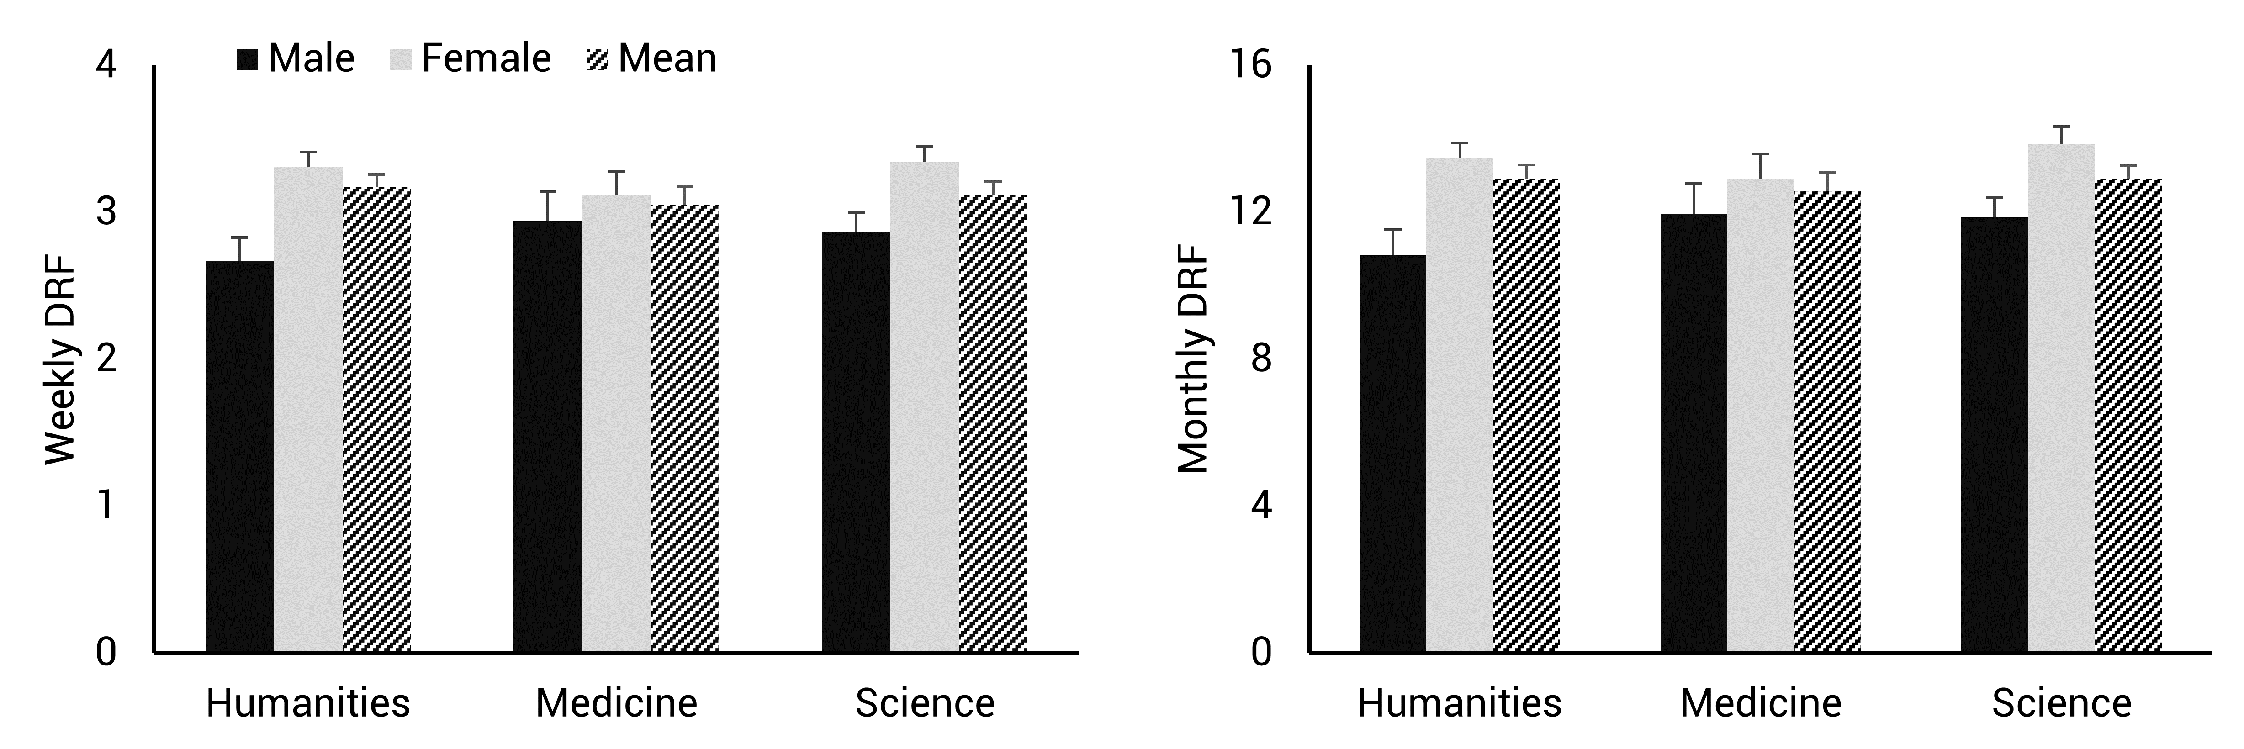
\includegraphics[width=\textwidth]{Fig/Results/Survey/S1_Fig.png}
	\caption*{\textbf{S1 Fig. Dream recall frequency as a function of gender and academic disciplines.} Left: weekly DRF (number of mornings per week with a dream in mind), Right: monthly DRF (number of mornings per month with a dream in mind). Error bars represent standard error.}
\end{figure}
